\documentclass[a4,center,fleqn]{NAR}

% Enter dates of publication
\copyrightyear{2008}
\pubdate{31 July 2009}
\pubyear{2009}
\jvolume{37}
\jissue{12}

%\articlesubtype{This is the article type (optional)}

% my imports
\usepackage{booktabs} 
\usepackage{colortbl} 
\usepackage{xcolor} 
\usepackage{xfrac}
\usepackage{multirow}
\usepackage{siunitx}

\begin{document}

\title{PK-DB: PharmacoKinetics DataBase for individualized and stratified computational modeling}

\author{%
Jan Grzegorzewski\,$^{1}$,
Janosch Brandhorst\,$^{1}$
Dimitra Eleftheriadou\,$^{1}$
Kathleen Green\,$^{2}$
Matthias Koenig\,$^{1}$%
\footnote{To whom correspondence should be addressed.
Tel: +44 000 0000000; Fax: +44 000 0000000; Email: xxx@yyyy.ac.zz}}

\address{%
$^{1}$Institute for Theoretical Biology, Humboldt University Berlin, Berlin, Germany
and
$^{2}$Department of Biochemistry, Stellenbosch University, Stellenbosch, South Africa}
% Affiliation must include:
% Department name, institution name, full road and district address,
% state, Zip or postal code, country

\history{%
Received January 1, 2009;
Revised February 1, 2009;
Accepted March 1, 2009}

\maketitle

\begin{abstract}
  There is plenty of data in pharmacokinetics literature which could be taken advantage of with computational modeling in systems biology and systems medicine. Data integration prerequisites a standardized data representation but so far there is no open solution for reproducible and reusable storage of pharmacokinetics data. We present PK-DB, a database for pharmacokinetics data and information from clinical trials as well as pre-clinical research. PK-DB provides curated pharmacokinetics data integrated with the corresponding meta-information (i) characteristics of studied patient collectives and individuals (e.g., age, body weight, smoking status); (ii) applied interventions (e.g., dosing, substance, route of application); and (iii) measured pharmacokinetics time-courses and pharmacokinetics parameters (e.g., clearance, half-life, area under the curve). Important features are the representation of experimental errors and variation, the representation and normalisation of units, annotation of information to biological ontologies, calculation of pharmacokinetics information from concentration-time profiles (e.g., apparent clearance, half-life, area under the curve (AUC)), a workflow for collaborative data curation, strong validation rules on the data, and a simple access via a REST API. A special focus of PK-DB is the curation of data and meta-data for individualized and stratified computational modeling with methods like physiologically based pharmacokinetic (PBPK), pharmacokinetic/pharmacodynamic (PK/DB), or population pharmacokinetic (pop PK) modeling. We demonstrate the value of PK-DB via a stratified meta-analysis of pharmacokinetics studies for caffeine curated from literature which allows us to integrate and harmonize pharmacokinetics information from a wide range of studies and sources.
\end{abstract}


\section{INTRODUCTION}
 \textbf{Pharmacokinetics and Data} The Pharmacokinetics (PK) of drugs and medication are of great interest in medical research and drug development. The main measures in the field are concentration-time profiles and corresponding PK parameters like half-life or clearance rate. These measures strongly depend on the dosage and individual characteristics of the subject under investigation. Individual and population-related information such as age, weight, sex or disease status drives inter-individual variability \cite{Polasek2018} which makes them indispensable for the research of pharmacokinetics. The study of variability in drug exposure due to these covariates is a big field of research with a long history. It is generally referred to as population pharmacokinetics \cite{Aarons1991}. Modern approaches go beyond classical population information by accounting for genetic variation \cite{Lotsch2006} and other more hidden variables. This kind of subject information in combination with the main measures are the foundation for an individual approach in drug treatment which will potentially pave the road towards precision dosing and precision medicine. % something to industrialization of PK \cite{Romero2010}
\par 
A multitude of publications have been written about pharmacokinetics studies but despite the wealth of reported data in the literature and the requirement for pharma-companies to perform such experiments before bringing drugs on the market almost none of the data is publicly accessible in a machine-readable format and certainly not with FAIR (findable, accessible, interoperable and reproducible) \cite{Wilkinson2016} principles in mind. The only way to retrieve this treasure is by digitizing and curating this information from publications. Despite the central role of pharmacokinetics information in the medical and pharma field, or perhaps exactly because of that, no open freely accessible database of pharmacokinetics information exists so far. Heterogeneity in the reporting of clinical study designs, pharmacokinetic measures, individual, and population-related meta-information complicates data integration. For computational modeling, meta-analysis, and most methods in machine learning and artificial intelligence a standardized and machine-readable representation of data is of major importance. PK data can be utilized in many different ways  \cite{Mould2012,Mould2013,Upton2014}. 
Physiologically based pharmacokinetic models (PBPK) provide a unique opportunity to translate different PK parameters from multiple clinical trials into one model. The mechanistic models can account for the differences in the study protocol, dosing, and individuals and population characteristics. 
Here we present PK-DB a database for pharmacokinetics information with a special focus on storing information for individualization and stratification of computational models.


% **************************************************************
% Keep this command to avoid text of first page running into the
% first page footnotes
%\enlargethispage{-65.1pt}
% **************************************************************

\section{DESCRIPTION \& RESULTS}

\subsection{Design and Technology}

Key principles in the design of PK-DB were \textbf{(i) accessibility of data for computational modeling and data science.} Biologically motivated data like substances or diseases are annotated to biological ontologies. This enables the integration with other data sets and computational models, e.g., substances to ChEBI \cite{Hastings2016}, and diseases to ncit, hp, doid, and mondo \cite{Sioutos2007, Kohler2019, Kibbe2015, Mungall2017}. PK-DB was designed as a web-reachable database, accessible either via a web frontend or programmatically via a REST API. Hereby, most of the data is indexed for a fast full-text search; 
\textbf{(ii) extensibility and generalizability}, the data model is not focused on a narrow problem domain but allows simple extensions to other fields and experimental data sets, within the overall domain of pharmacokinetics. Good examples are extensible types for the group or individual characteristics. Additional types can easily be added to cover the important information for a given problem domain;
\textbf{(iii) tracking changes in curated data} and allowing an intuitive and collaborative multi-curator curation;
\textbf{(iv) unit and data normalization}, a key challenge in using data for computational modeling and data science are non-standardized units coming from different data sets. It requires time-consuming retrieval of this information from the literature and error-prone conversion of units and corresponding data. PK-DB provides a solution to this issue. During upload the data is harmonized, e.g., data is converted between molar units and gram, using thereby the molecular mass of the respective substances based on its ChEBI information  \cite{Hastings2016};
\textbf{(v) representation of time-course data}, the main measures in pharmacokinetics studies are concentration-time curves of the administered substance and its metabolites after biotransformations. These time-courses are crucial for kinetic modeling, e.g., using physiologically based pharmacokinetic (PBPK) or pharmacokinetics/pharmacodynamics (PK/PD) models. On study upload, PK-DB is automatically calculating important secondary PK parameters such as AUC, half-life, clearance or volume of distribution from the time-concentration profiles; 
\textbf{(vi) high data quality}, strong validation e.g. of categoricals, minimum relevant information, instance cross-referencing and correct unit-dimensions ensure high curation quality. Nonobvious curation mistakes can be addressed by outlier identification in subsequent meta-analyses.
PK-DB allows to keep studies privately or only share with certain collaborators. This allows sharing the study during the curation process only with trusted people with a simple option to make the study public at any time. Some information is only available to a limited group of people due to copyright issues, e.g., for manually curated studies from the literature the underlying publication can only be made accessible if it is Open Access.
\par
The PK-DB backend is using Django and is written in python. The database is based on Postgres. It is accessible at \url{https://pk-db.com/api/} via a REST API based on the Django-rest-framework. Most data is indexed with elastic search enabling fast, full-text search. The search endpoints are part of the single REST API. Major advantages of a REST API as a central access point to the database is that it can be accessed from multiple clients independent of the programming language. In the following, various use cases demonstrate the usefulness of our approach. First, internally the API is used by a web frontend which enables a human-friendly interaction with the data. The frontend is implemented in javascript based on vue.js and can be accessed at \url{https://pk-db.com}. 
Further, the endpoint can be accessed programmatically which allows the integration of data with computational models, for meta-analyses and data science in general. Running analysis scripts against the database in python, or creating overview plots of the database content using R (circos) gets very feasible. In figure \ref{NAR-fig4}, we show an exemplary meta-analysis of caffeine clearance rates stratified into different subgroups depending on lifestyle factors and pooled from multiple studies via the  REST API. Also, the data manipulation goes via the  REST entry point.

\subsection{Curation workflow \& minimal information for pharmacokinetics data}
A python package (pkdb\_data) provides an interface for an easy curation workflow.  It simplifies the uploading, updating, and deleting of the curated data into the database. Locally it provides a repository with a representation of the data as single files. During the curation workflow, the corresponding files can be automatically validated on save with the feedback being printed in the terminal. This allows the curator to perform changes to files with direct feedback about allowed choices. Many constraints are added on the validation layer instead of having the data model layer too restrictive.
The typical workflow for extracting data from the literature is depicted in figure \ref{NAR-fig1}. Before the curation process, typically initial literature research for a given problem domain has to be performed, resulting in a corpus of papers for curation. Within the curation process, the relevant information is manually extracted from the literature and encoded in a study.json format.  
We decided for a simple JSON format in the main document and optional tabular data. The tabular data can be parsed into the main document. This comes especially handy for studies with large datasets. Such a simple format allows tracking changes easily via version control based on git. Curation is an iterative process with often changing curators over time. Tracking changes to the curated data is crucial. Instead of implementing such history and change tracking on database level with substantial overhead, we can utilize the full set of git features out of the box to track changes to our files. There is no need for a secondary curation frontend. We can curate data while we develop the database without the need to maintain a full frontend for curation.

\begin{figure}[t]
\begin{center}
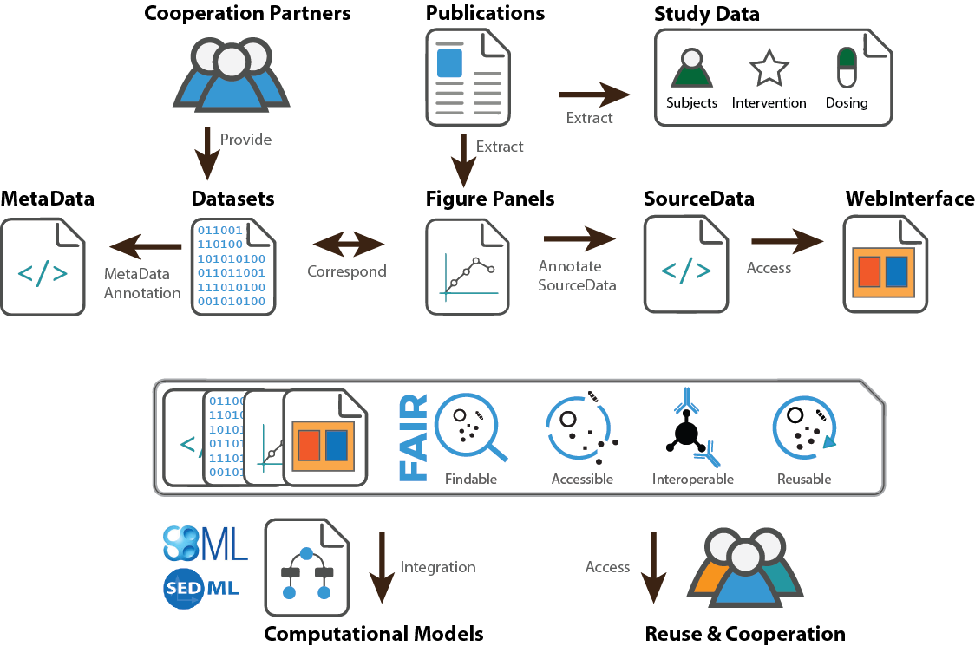
\includegraphics{NAR-fig1.png}
\end{center}
\caption{\textbf{Data curation workflow}. This figure shows schematically the curation process. (i) Data is either extracted from literature or integrated from clinical partners. (ii) Data is coded into the study.json format and uploaded to PKDB. During the process, the curated data is validated. After the upload, the data can be accessed either via the web frontend or via the REST API.}
\label{NAR-fig1}
\end{figure}

\subsection{Calculation of pharmacokinetics parameters}
An important part of PK-DB is the automatic calculation of pharmacokinetic parameters from the reported concentration-time curves. These most prominent pharmacokinetic parameters are calculated based on non-compartmental methods \cite{Gabrielsson2012}. Calculated parameters are the area under the curve (\si{AUC_{end}}), the area under the curve extrapolated to infinity (\si{AUC_{\infty}}), the concentration maximum (\si{C_{max}}), the time at concentration maximum (\si{t_{max}}), the half-life (\si{t_{half}}), the elimination rate (\si{k_{el}}), the clearance (\si{clearance}) and the volume of distribution (\si{Vd}). Figure \ref{NAR-fig2} and table \ref{table:01} illustrate the automatic calculation of the prominent PK parameters from concentration-time profiles. Here, the data originates from a study on the influence of specific genetic alleles on the pharmacokinetics \cite{Wu2014}. No individual participants data (IDP) but averaged measures with variation were reported. Mathematically strict, first the PK parameters should be calculated for each participant individually and finally averaged which is not possible if only averaged data is reported. This is the reason for the notable difference between reported and calculated Pks displayed in table \ref{table:01}. Even more fundamentally, the description of the data as averages with variations often hinges. This description hiddenly assumes homogeneity of the data which often is not the case \cite{Hanin2017}. Therefore, we strongly encourage to publish IDPs. Often only a subset of the prominent pharmacokinetic information is reported. In this study e.g., the volume of distribution and the elimination rate were initially not reported but automatically calculated by PK-DB.

\begin{figure}[t]
\begin{center}
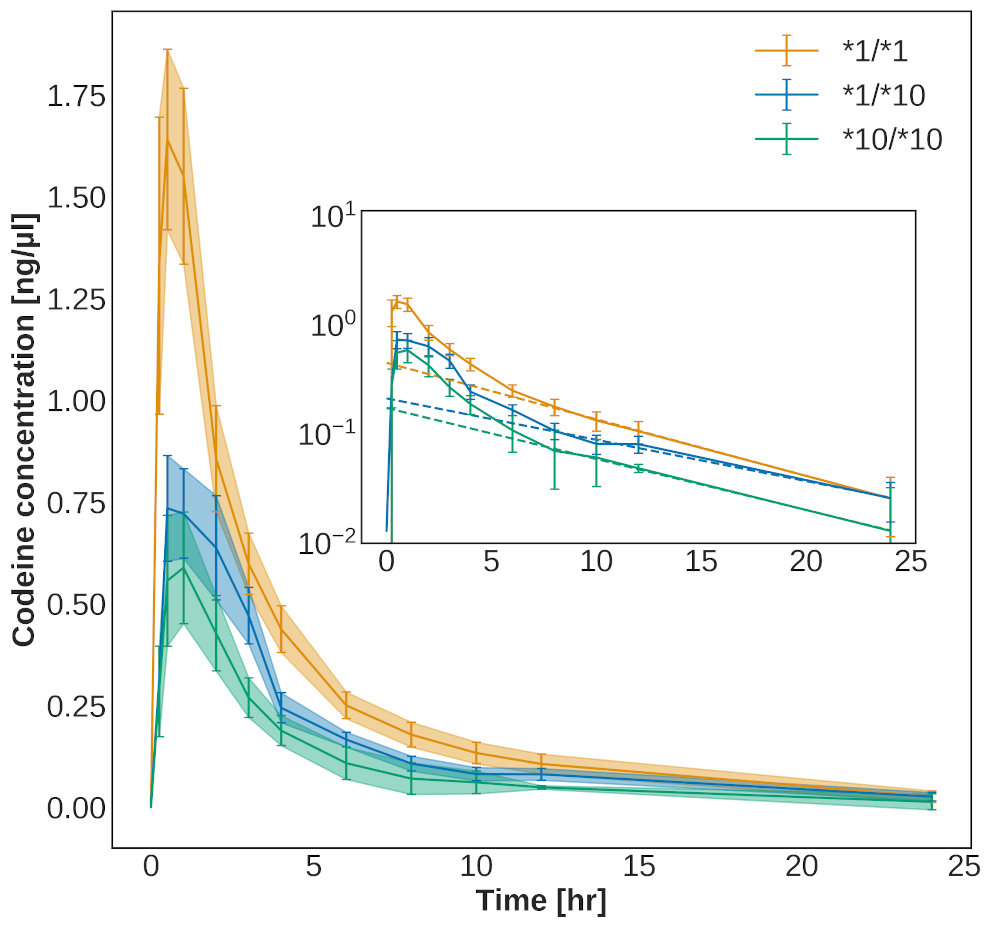
\includegraphics{NAR-fig2.png}
\end{center}
\caption{\textbf{Calculation of pharmacokinetics data from time-courses.} \newline
Pharmacokinetics parameters are calculated from reported concentration-time profiles using non-compartmental methods. The figure displays paradigmatic concentration profiles reported as averages with a standard error. Here, they are taken from the literature and correspond to three subgroups with different genetics \cite{Wu2014}. The calculated and reported PK parameters are displayed and compared to each other in table \ref{table:01}. Due to the unavailability of individual participant data in most pharmacokinetics studies parameters are determined on the averages of the time-concentration curves.
}
\label{NAR-fig2}
\end{figure}

\begin{table}
\tableparts{%
\caption{\textbf{Reported and calculated PKs} The table shows the most prominent PK parameters reported in a pharmacokinetics study on three subgroups with different genetics \cite{Wu2014}. Pks calculated and reported by the authors are compared to the Pks calculated by PKDB from the concentration-time profiles in figure \ref{NAR-fig2}, which were also reported by the authors. No individual data were reported, which results in the differences in the values.}
\label{table:01}%
}{%
\begin{tabular*}{\columnwidth}{@{}ll|ll|l@{}}
\toprule
Measurement type & Genotype & Reported & Calculated & Rel. dif.
\\
(unit)& & \si{\overline{x_{r}} \pm std(x)} &  \si{\overline{x_{c}}} & \si{\frac{\overline{x_{r}} - \overline{x_{c}}}{0.01 \cdot \overline{x_{r}}}} \\
&  &  &  & (\%) \\
\colrule
\si{AUC_{END}}              & *1/*1  &6.63 $\pm$ 2.07& 6.24  & 5.88 \\ 
(\si{ng \per \mu l \c.hr})  & *1/*10 & 3.77$\pm$  1.93& 3.8    &  -0.8 \\ 
                            & *10/*10 & 2.65$\pm$ 1.95& 2.59  & 2.26 \\
\colrule
\si{AUC_{\infty}}              &  *1/*1  & 8.52 $\pm$ 4.10 & 6.4  & 24.88 \\ 
(\si{ng \per \mu l \c.hr})  & *1/*10  & 5.05 $\pm$ 3.30& 3.97  & 21.39 \\ 
                            & *10/*10 & 3.26 $\pm$  2.43& 2.68  & 17.79 \\
\colrule
\si{Clearance}              &  *1/*1   &5.08 $\pm$ 3.39& 5.24  & -3.158 \\ 
(\si{l \per hr})  &  *1/*10  &9.72 $\pm$ 8.72& 8.02  & 17.49 \\ 
                           &  *10/*10 & 16.20 $\pm$ 12.30& 13.1  & 19.14 \\
\colrule
\si{C_{max}}              & *1/*1   & 2.06$\pm$  0.89& 1.64 &  20.39 \\ 
(\si{hr})  & *1/*10  &0.96 $\pm$ 0.42& 0.73 &  23.96 \\ 
                          & *10/*10 &0.68 $\pm$ 0.50& 0.59 &  13.24 \\
\colrule
\si{t_{half}}              & *1/*1   & 9.40$\pm$ 11.70& 4.15 &  55.85 \\ 
(\si{hr})  & *1/*10  &11.50 $\pm$ 11.10& 4.76 &  58.61 \\ 
                          & *10/*10 & 6.84 $\pm$  5.46 & 4.66 &  31.87 \\
\colrule
\si{t_{max}}              & *1/*1   & 0.64 $\pm$ 0.28 & 0.5 &  21.88 \\ 
(\si{hr})   & *1/*10  & 0.86 $\pm$ 0.52 & 0.5 &  41.86 \\ 
                          & *10/*10 & 0.86 $\pm$ 0.52 & 1   &  -16.28 \\
\colrule
\si{Vd}              & **1/*1 & -- & 31.3 & -- \\ 
(\si{l})   & *1/*10 & -- & 55 & -- \\ 
                          & *10/*10 & -- & 88.1 & -- \\
\colrule
\si{k_{el}}              & *1/*1 & -- & 0.17 & -- \\ 
(\si{1 \per hr})   & *1/*10 & -- & 0.15 & -- \\ 
                          & *10/*10 & -- & 0.15 & -- \\
\botrule
\end{tabular*}%
}
{data is presented as mean $\pm$ standard deviation \par
 Not reported or  not calculable  values are  displayed as (--)
}
\end{table}

\subsection{Statistics}
The current focus of the data curation lies in clinical studies for substances used in dynamical liver function tests as well as for the modeling of the whole-body glucose metabolism. In the current state, PK-DB-v0.7.0 consists of 183 studies containing 473 groups, 1808 individuals, 510 interventions, 15790 outputs and 1260 time-courses related to caffeine, glucose, codeine, or paracetamol (see Figure \ref{NAR-fig3} and for the full picture Figure\_S1, Figure\_S2, and Table\_S3 in the supplements).


\begin{figure*}[t]
\begin{center}
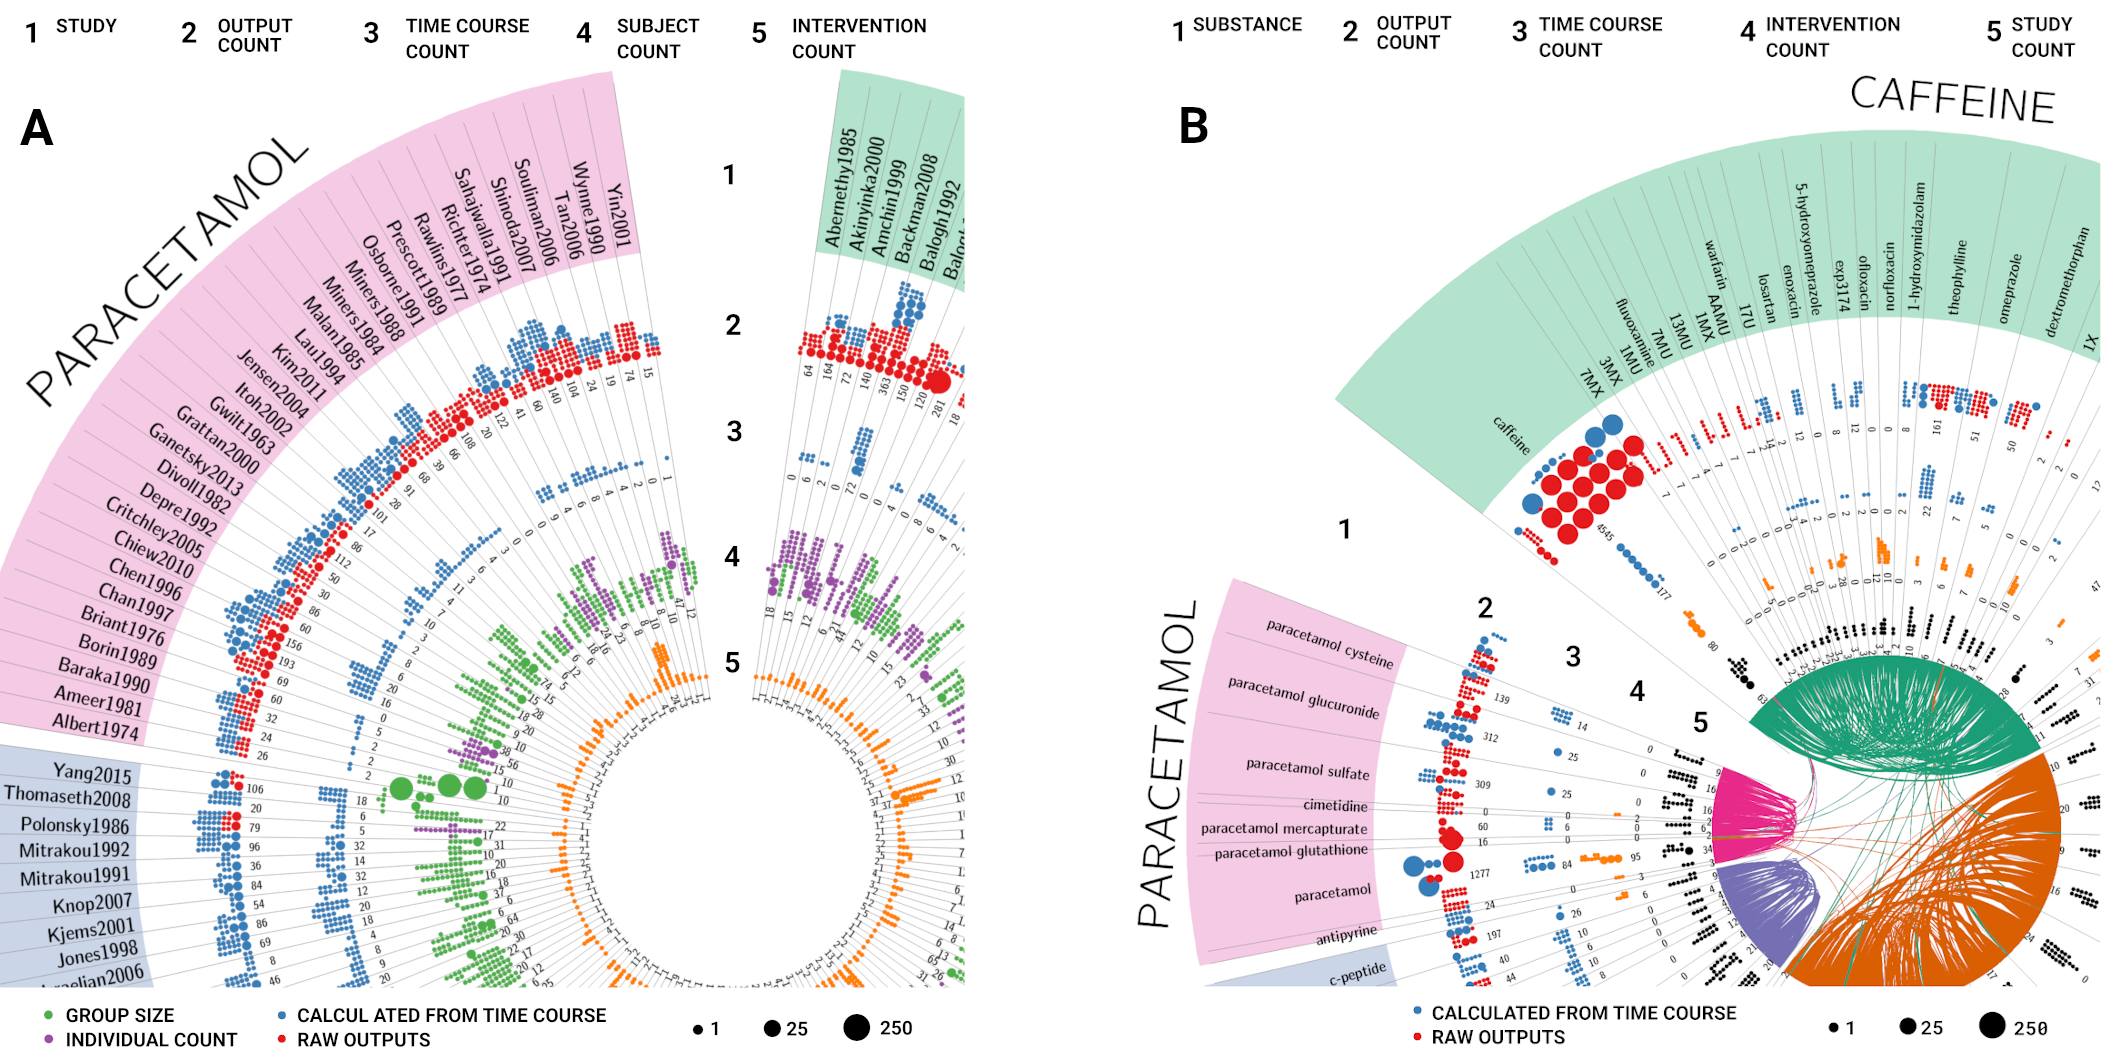
\includegraphics{NAR-fig3.png}
\end{center}
\caption{Database content overview
\textbf{ A) Study overview} The figure shows a fraction of the current studies in the database. The complete corresponding data is provided in SUPPLEMENT\_TAB1 and visualized in SUPPLEMENT\_FIG1. PK-DB-v0.7.0 consists of 183 studies containing 473 groups, 1808 individuals, 510 interventions, 15790 outputs and 1260 time-courses related to caffeine, glucose, codeine, or paracetamol. The circular plot is structured in stripes and rings. Each stripe represents a different study. In each ring, the amount of different data types for the respective study is depicted. The dots represent the respective amount of data with the dot size corresponding to the number of entries per dot. The rings describe the following information for the respective study (1) name of the study; (2) number of outputs (pharmacokinetics parameters and other measurements). Red dots represent reported data, blue dots data calculated from time-courses reported in the study; (3) number of time-courses; (4) number of participants. Purple dots represent participants with individual data (IPD), green dots represent participants which are reported as a group; (5) the number of interventions applied to the participants in the study.
\textbf{ B) Substance overview} The figure shows a fraction of the current substances in the database. Substances with few entries are excluded from the plot. The circular plot is structured in stripes and rings. Each stripe represents a different substance. In each ring, the amount of different data types for the respective substance is depicted. The figure is classified into 5 substance classes (caffeine, glucose, codeine, and paracetamol). The classification is performed by agglomerative clustering of the pair co-occurrence of substances within studies. The names for the classes are chosen to be the names of the most frequent substance within the class. Each co-occurrence of two substances is visualized by a connecting ribbon in the center of the figure. The dots represent the respective amount of data with the dot size corresponding to the number of entries per dot. The rings describe the following information for the respective substance (1) name of the substance; (2) number of outputs (pharmacokinetics parameters and other measurements). Red dots represent reported data and blue dots represent data calculated from reported concentration-time profiles. (3) the number of time-courses; (4) number of applied interventions; (5) number of studies in which the substance was used.
}
\label{NAR-fig3}
\end{figure*}

\subsection{Meta-analysis of caffeine}
In the following, a use case is presented demonstrating the programmatic interaction with PK-DB.
PK-DB allowed us for the first time for an extensive and systematic analysis of the effect of lifestyle factors like smoking and oral contraceptive use on the clearance of caffeine. We integrated data from 44 studies. By curating information about the respective patient characteristics (lifestyle factors), the actual interventions performed in the studies (dosing and route), and important information like the errors on the reported data we could gain a unique view on the strong and consistent effect of smoking and oral contraceptive use on the clearance of caffeine. 
Importantly, the meta-analysis allowed us to directly improve the curation status of many studies by easily visually detecting outliers in the data which could in most cases directly be backtracked to curation errors which could subsequently be corrected. 
A positive point is that most of the reported studies are consistent. For instance with caffeine, most of the data was in line with each other with a single exception being Stille1987 \cite{Stille1987}. Here a systematic bias in the data could be observed probably due to an analytic problem. Besides, problems existed with reporting the same data set multiple times, overall in four publications \cite{Stille1987, Harder1988, Harder1989, Balogh1992}. The extreme variability between studies and individuals could be markedly reduced by accounting for lifestyle information.
\subsection{Data quality and validation}
The integration of data from multiple studies and subsequent meta-analyses is a valuable procedure to identify curation errors which cannot be caught by the validation rules. The combination of both, the validation rules and the meta-analyses helped to identify errors also in the reporting. In the following, we will give some examples of suspicious reported data. 
\textbf{(i)} In the study Wang1985 \cite{Wang1985} units have been reported incorrectly. 
\textbf{(ii)} In Seng2009 \cite{Seng2009} volumes per body weight have been calculated incorrectly. 
\textbf{(iii)} In Balogh1992, Harder1988, Harder1989 and Stille1987 \cite{Stille1987,Harder1988, Harder1989,Balogh1992} probably the same data was reported. Suspiciously 10mg difference in dosing was reported. Furthermore, the data is not fitting into other datasets of the meta-analysis of caffeine. It is unclear if this is a reporting error or due to something else e.g. assay bias, hidden covariates.
\textbf{(iv)} In Carbo1989 \cite{Carbo1989} participant number 4 has a suspiciously high half-life and participant number 3 a suspiciously high clearance rate. It is unclear if this is a reporting error.
\textbf{(v)} In Beach1986 \cite{Beach1986} 9 smokers and 2 non-smokers have suspiciously very high clearance rates, again unclear if this is a reporting error. 
\textbf{(vi)} In Wu2014 \cite{Wu2014} the concentration-time profiles and concentration maxima were reported with the wrong unit.

\begin{figure*}[t]
\begin{center}
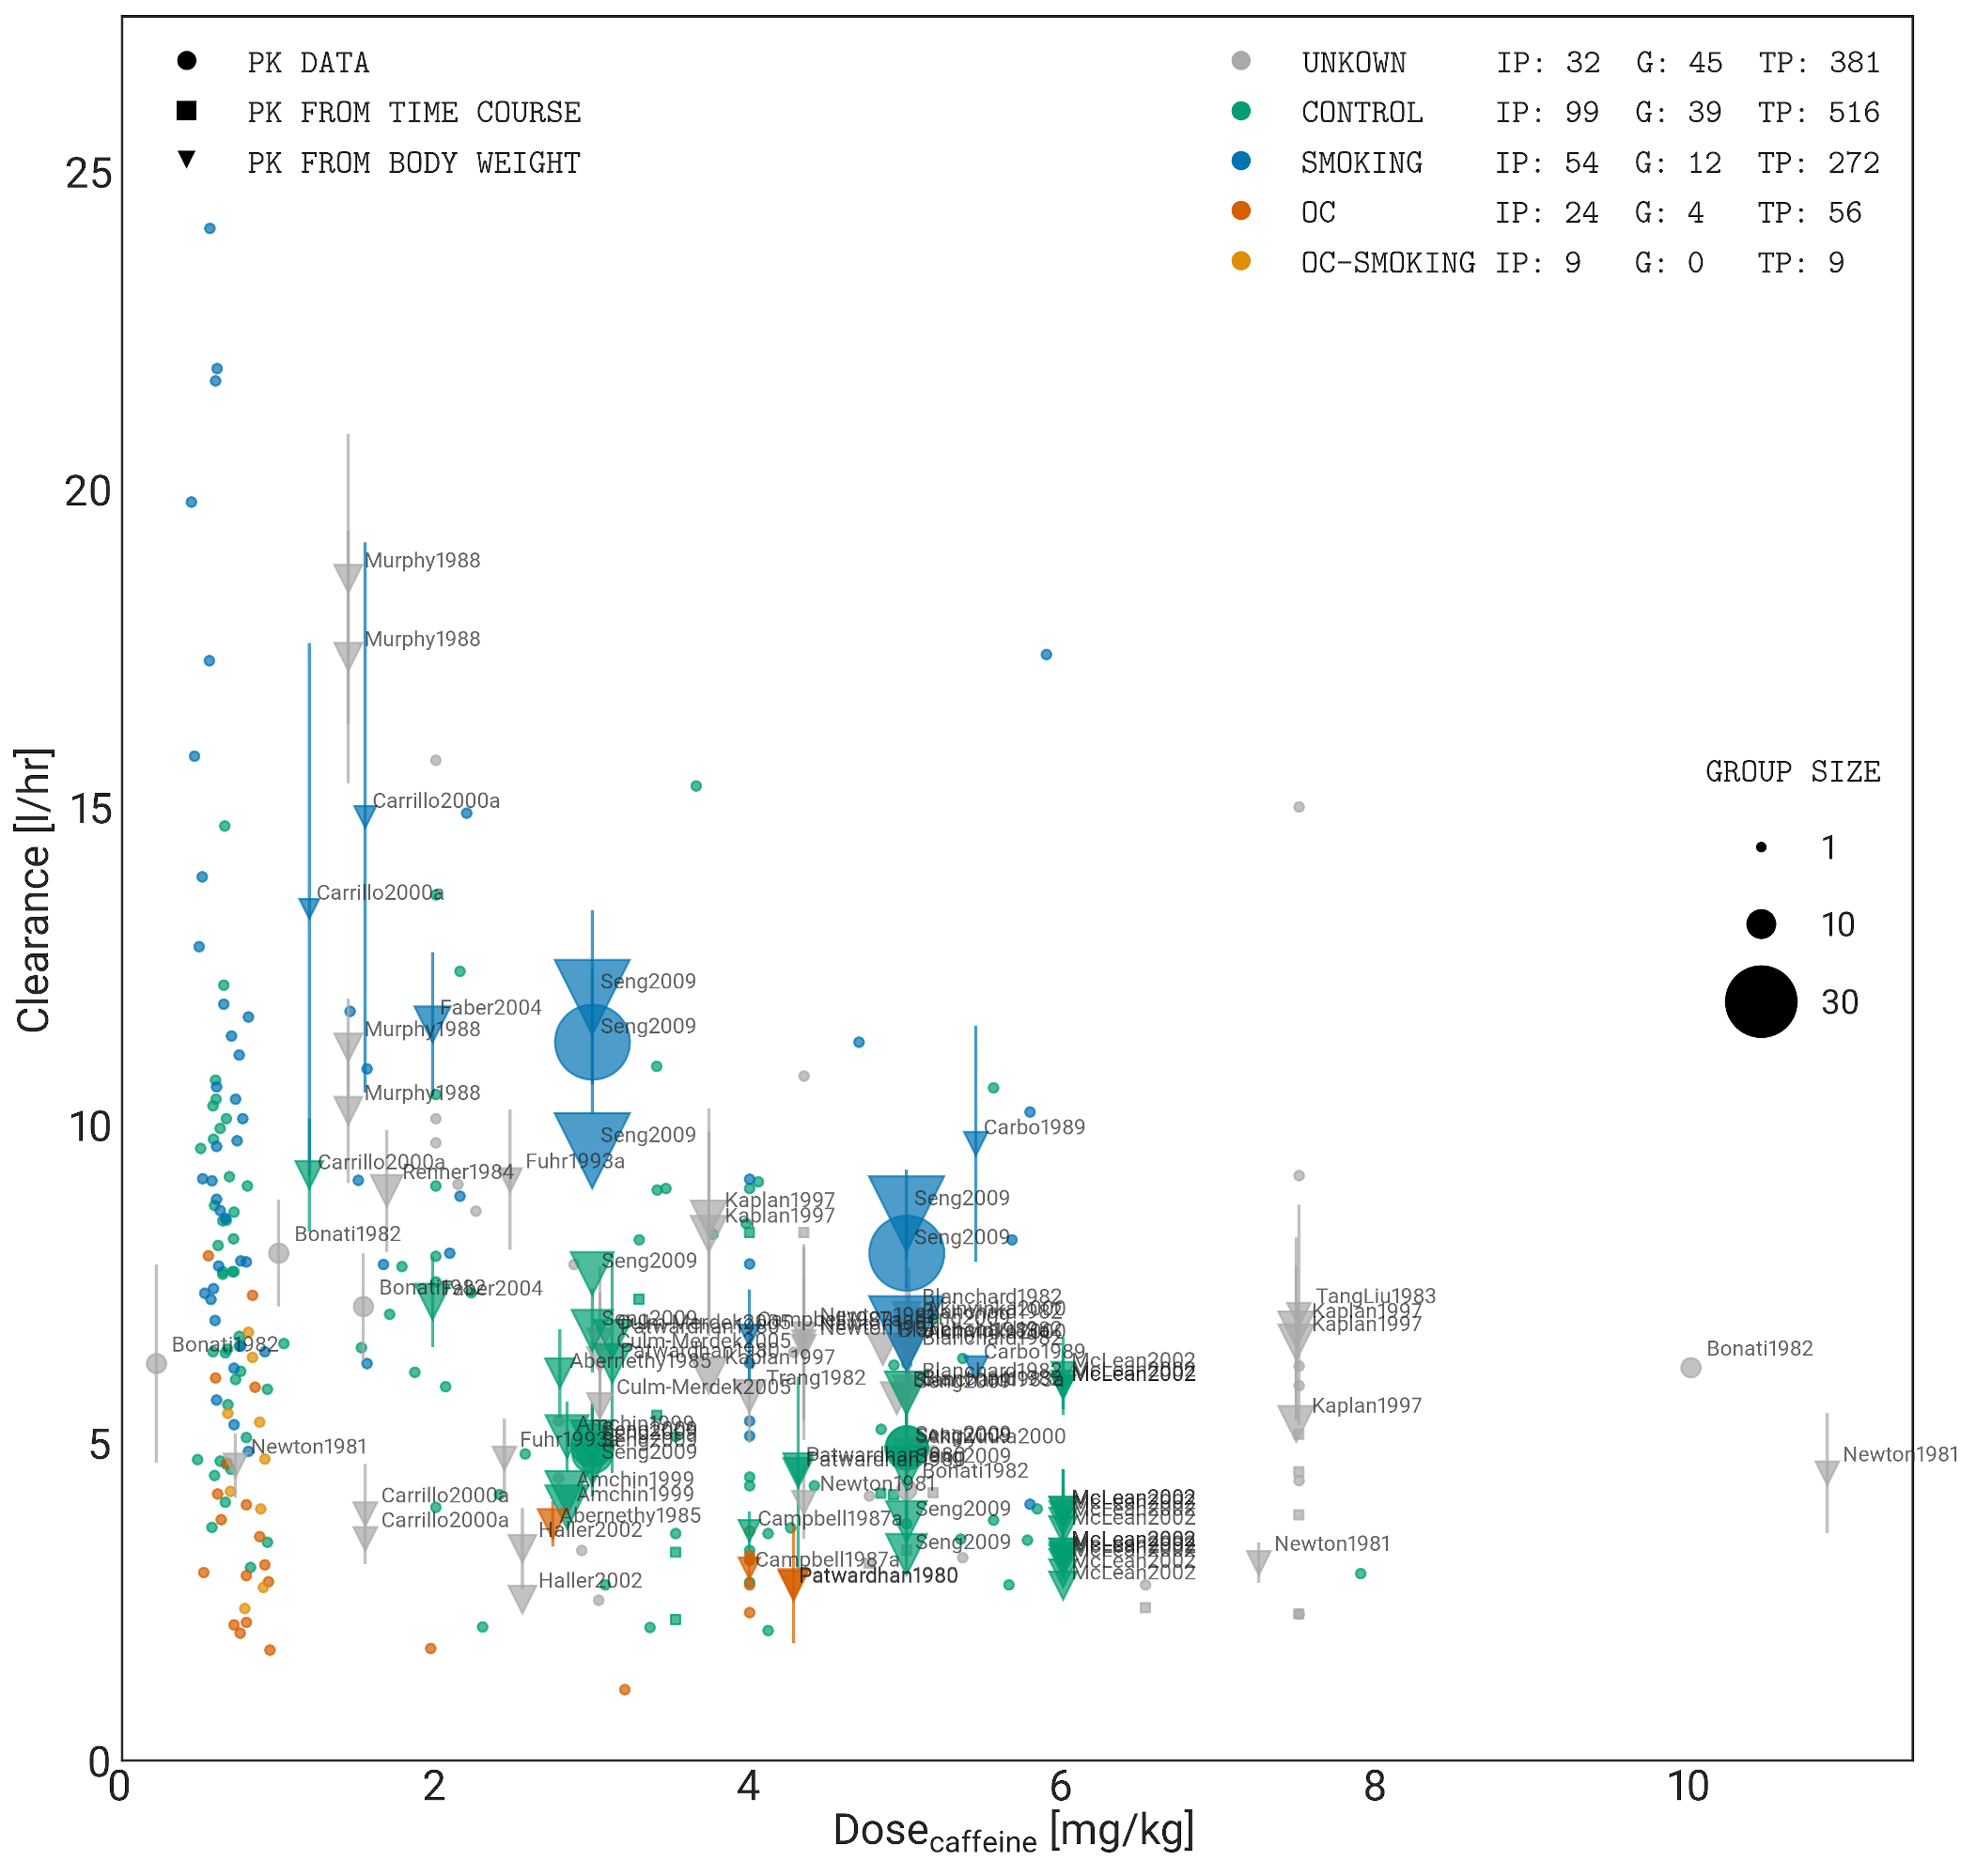
\includegraphics{NAR-fig4.png}
\end{center}
\caption{\textbf{A meta-analysis of caffeine clearance rates vs. caffeine dose} \newline
 The data is stratified based on reported smoking and oral contraceptive (OC) use. UNKNOWN (grey) data corresponds to unreported smoking and OC, CONTROL (green) are non-smokers, not taking OC, SMOKING (blue) are smokers and not taking OC, OC (dark orange) are non-smokers taking OC, and OC-SMOKING (light orange) to smokers taking oral contraceptives. Individual and group data with group size depicted as dot size is displayed. In the legend, (IP), (G) and (TP) stands for individual participants, the number of groups and total participants, respectively. Data points coming from groups are labeled by the name of the study from which they originate. Data points are depicted as circles if reported similar in the study, as squares if calculated from concentration-time profiles and as triangles if inferred from corresponding pharmacokinetic data and the body weights of the participants. Typically dosing is reported in mass units and clearance in a volume per time. Sometimes both values are reported in body weight units. Here, all available data is harmonized. Suspicious data from four studies \cite{Stille1987, Harder1988, Harder1989, Balogh1992} coming probably from the same clinical investigation was excluded.
}
\label{NAR-fig4}
\end{figure*}
\section{CONCLUSION \& DISCUSSION}

PK-DB is the first publicly available database for pharmacokinetics data. We could demonstrate the value of PK-DB by performing a meta-analysis of available studies on caffeine clearance. The database allows based on the data model and integration of study information like dosing and group information the stratification and individualization of the available data sets.
By providing the first open database for pharmacokinetics information we provide an important resource which allows storing pharmacokinetics information in a FAIR (findable, accessible, interoperable and reproducible) manner. 
By performing the data curation for commonly apply drugs (codeine and paracetamol), a substance used in liver function tests (caffeine) and a well-studied substance (glucose) we could gain insights into how well data is reported in the various fields.

In summary, the reporting of data is very poor despite the main point of the publications being the reporting of the data. Without guidelines on minimal information for studies, it is very difficult to compare studies or integrate data from different sources. Minimal guidelines about reporting patient characteristics for individuals and groups which is lacking in most of the studies. Incomplete and poor reporting of data in the field of pharmacokinetics has been reported also by others \cite{Kanji2015, Dykstra2015}.
Based on our work we have a set of important suggestions when publishing clinical studies in the field of pharmacokinetics. \textbf{(i)} Publish the actual data in a machine-readable format (e.g., a data table in the supplement). \textbf{(ii)} Provide the data for individual subjects (IPD) which is much more informative and allows to calculate all data for the groups. Most studies only report group averaged time-courses data and often not even errors on the data is reported. \textbf{(iii)} Provide minimum information on patient characteristics which includes basic anthropometric information like age, body weight, sex, height, and the subset of important lifestyle factors known to alter pharmacokinetics, e.g. co-medication, oral contraceptive use, smoking status, alcohol consumption or for instance for CYP1A2 substrates like caffeine: methylxanthine consumption/abstinence. \textbf{(iv)} Clearly state the study protocol: Which substance was given in which dose, in which route (oral, intravenous), and in which form (tablet, capsule, solution), the more specific the information the better.
As our analysis shows, that even the basic pieces of information are not reported in many publications. It is impossible to integrate such data. An example is, for instance, codeine, where often not even the given dose can be retrieved because it is unclear which type of substance was administered to the body (codeine-sulfate, codeine-phosphate or the actual codeine). 







\section{ACKNOWLEDGEMENTS}
Funding: JG and MK are supported by the Federal Ministry of Education and Research (BMBF, Germany) within the research network Systems Medicine of the Liver (LiSyM, grant number 031L0054).

\subsubsection{Conflict of interest statement.} None declared.
\subsubsection{Contributions:}
\newpage
\begin{thebibliography}{4}

% Format for article
\bibitem{Polasek2018}
Polasek, Thomas M.,Shakib, Sepehr and Rostami-Hodjegan, Amin  (2018)
Precision dosing in clinical medicine: present and future
\textit{ Expert rev. clin. Phar.}, \textbf{11(8)}, 743--746.

% Format for article
\bibitem{Aarons1991}
Aarons, L. (1991)
Population pharmacokinetics: theory and practice.
\textit{Br. J. Clin. Pharmacol.}, \textbf{32(6)}, 669--670.

% Format for article
\bibitem{Lotsch2006}
Loetsch, Joern, Skarke, Carsten, Schmidt, Helmut, Rohrbacher, Maren, Hofmann, Ute, Schwab, Matthias and Geisslinger, Gerd  (2006)
Evidence for morphine-independent central nervous opioid effects after administration of codeine: Contribution of other codeine metabolites
\textit{Clin. Pharm. Ther.}, \textbf{79(1)}, 35--48.

% Format for article
\bibitem{Wilkinson2016}
Wilkinson et al. (2016)
Comment: The FAIR Guiding Principles for scientific data management and stewardship
\textit{  Sci. Data}, \textbf{3}, 1--9.% Format for article

% Format for article
\bibitem{Mould2012}
Mould, D. R. and Upton, R. N. (2012)
Basic concepts in population modeling, simulation, and model-based drug development
\textit{ CPT Pharmacometrics Syst. Pharmacol.}, \textbf{1(1)}, 1--14.

% Format for article
\bibitem{Mould2013}
Mould, D. R. and Upton, R. N. (2013)
Basic concepts in population modeling, simulation, and model-based drug development - Part 2: Introduction to pharmacokinetic modeling methods
\textit{ CPT Pharmacometrics Syst. Pharmacol.}, \textbf{2(4)},

% Format for article
\bibitem{Upton2014}
Upton, R. N. and Mould, D. R. (2014)
BBasic concepts in population modeling, simulation, and model-based drug development: Part 3-introduction to pharmacodynamic modeling methods
\textit{ CPT Pharmacometrics Syst. Pharmacol.}, \textbf{3(1)}, 1--16.

% Format for article
\bibitem{Hastings2016}
Hastings, Janna et al.  (2016)
ChEBI in 2016: Improved services and an expanding collection of metabolites
\textit{Nucleic Acids Res.}, \textbf{44(D1)}, D1214--D1219.

% Format for article
\bibitem{Sioutos2007}
Sioutos, Nicholas et al.  (2007)
NCI Thesaurus: A semantic model integrating cancer-related clinical and molecular information
\textit{J. Biomed. Inform.}, \textbf{40(1)}, 30--43.

% Format for article
\bibitem{Kohler2019}
Koehler, Sebastian et al. (2019)
Expansion of the Human Phenotype Ontology (HPO) knowledge base and resources
\textit{Nucleic Acids Res.}, \textbf{47(D1)}, D1018--D1027.

% Format for article
\bibitem{Kibbe2015}
Kibbe, Warren A. et al. (2015)
Disease Ontology 2015 update: An expanded and updated database of Human diseases for linking biomedical knowledge through disease data
\textit{Nucleic Acids Res.}, \textbf{43(D1)}, D1071--D1078.


% Format for article
\bibitem{Mungall2017}
Mungall, Christopher J. et al. (2017)
The Monarch Initiative: An integrative data and analytic platform connecting phenotypes to genotypes across species
\textit{Nucleic Acids Res.}, \textbf{45(D1)}, D712-D722.

% Format for chapter in book
\bibitem{Gabrielsson2012}
Gabrielsson, J. and Weiner, D. (2012)
Non-compartmental Analysis
In
Reisfeld, B. and Mayeno, A. N (eds),
\textit{Computational Toxicology: Volume I},
Humana Press, Totowa, NJ,
pp.\ 377--389.

% Format for article
\bibitem{Wu2014}
Wu, X. , Yuan, L., et al. (2014)
The impact of CYP2D6 polymorphisms on the pharmacokinetics of codeine and its metabolites in Mongolian Chinese subjects
\textit{Eur. J. Clin. Pharmacol.}, \textbf{70(1)}, 57--63.

% Format for article
\bibitem{Hanin2017}
Hanin, L. (2017)
Why statistical inference from clinical trials is likely to generate false and irreproducible results
\textit{BMC Med. Res. Methodol.}, \textbf{17(1)}, 1--12.

% Format for article
\bibitem{Stille1987}
Stille, W., Shah, P. M. et al. (1987)
Decrease of caffeine elimination in man during co-administration of 4-quinolones
\textit{J. Antimicrob. Chemother.}, \textbf{20(5)}, 729--734.




% Format for article
\bibitem{Harder1988}
Harder, S. et al. (1988)
4-Quinolones Inhibit Biotransformation of Caffeine
\textit{Eur. J. Clin. Pharmacol.}, \textbf{35(6)}, 651--656.


% Format for article
\bibitem{Harder1989}
Harder, S. Fuhr, U, Staib, AH, Wolff T. (1989)
Ciprofloxacin-caffeine: a drug interaction established using in vivo and in vitro investigations.
\textit{Am. J. Med.}, \textbf{87(5A)}, 89--91.


% Format for article
\bibitem{Balogh1992}
Balogh A1, Harder S, Vollandt R, Staib AH.  (1992)
Population pharmacokinetics: theory and practice.
\textit{Int. J. Clin. Pharmacol. Ther. Toxicol.}, \textbf{30},383--387.


% Format for article
\bibitem{Wang1985}
Wang, T., Kleber, G., Stellaard, F. and Paumgartner, G.  (1989)
Caffeine elimination: A test of liver function
\textit{Klin. Wochenschr.}, \textbf{63(21)}, 1124--1128.

% Format for article
\bibitem{Seng2009}
Seng, K. Y. ,Fun, C. Y. ,Law, Y. L. et al.  (2009)
Population pharmacokinetics of caffeine in healthy male adults using mixed-effects models. 
\textit{J. Clin. Pharm. Ther.}, \textbf{63(21)}, 1124--1128.

% Format for article
\bibitem{Carbo1989}
Carbó, M., Segura, J., De la Torre, R., Badenas, J. M. and Camí, J.  (1989)
Pharmacokinetic parameters: which are necessary to define a drug substance?
\textit{Clin. Pharm. Ther.}, \textbf{45}, 234--240.

% Format for article
\bibitem{Beach1986}
Beach, C. A. , Mays, D. C., Guiler, R. C., Jacober, C. H., and Gerber, N. (1986)
Inhibition of elimination of caffeine by disulfiram in normal subjects and recovering alcoholics\textit{Clin. Pharm. Ther.}, \textbf{39(3)}, 265--270.

% Format for article
\bibitem{Kanji2015}
Kanji, S., Hayes, M., Ling, A., et al. (2015)
Reporting Guidelines for Clinical Pharmacokinetic Studies: The ClinPK Statement 
\textit{Clin. Pharmacokinet. }, \textbf{54(7)}, 783--795.

% Format for article
\bibitem{Dykstra2015}
Dykstra, K., Mehrotra, N., Tornoe, C., To   et al.  (2015)
Reporting guidelines for population pharmacokinetic analyses. 
\textit{J. Pharmacokinetic. Phar.}, \textbf{42(3)}, 301--314.


% Format for article
\bibitem{Benet1984} % not jet cited
Benet, LZ.  (1984)
Pharmacokinetic parameters: which are necessary to define a drug substance?
\textit{ Eur. J. Respir. Dis. Suppl.}, \textbf{134}, 45--61.


\end{thebibliography}




\end{document}
